\documentclass{article}
\usepackage[T1]{fontenc}
\usepackage{lmodern}
\usepackage{graphicx}
\usepackage{amsmath,amssymb}
\usepackage[a4paper,margin=2cm]{geometry}
\usepackage[absolute,overlay]{textpos}
\setlength{\TPHorizModule}{1mm}
\setlength{\TPVertModule}{1mm}
\usepackage[indonesian]{babel}
\usepackage{hyperref}
\setlength{\emergencystretch}{2em}
% unit: Halaman 47

\begin{document}

% === Halaman 47 (llm) ===

\vspace{228.69mm}

\begin{verbatim}
def dekripsi_aes(cipherteks, kunci):
    kunci = kunci.encode()
    cipherteks = base64.b64decode(cipherteks)
    iv = cipherteks[:16]
    AEScipher = AES.new(kunci, AES.MODE_CBC, iv)
    plainteks = AEScipher.decrypt(cipherteks[BLOCK_SIZE:])
    plainteks = unpad(plainteks, BLOCK_SIZE)
    return plainteks

# Program utama (pemanggilan fungsi enkripsi dan dekripsi AES)
# Enkripsi pesan
print("E N K R I P S I:")
pesan = input("Ketikkan pesan yang akan dienkripsi:")
kunci = input("Ketikkan kunci (harus sepanjang 16 karakter):")
cipherteks = enkripsi_aes(pesan, kunci)
print("Cipherteks hasil enkripsi: ", cipherteks)

# Dekripsi pesan
print("D E K R I P S I:")
kunci = input("Ketikkan kunci (harus sepanjang 16 karakter):")
plainteks = dekripsi_aes(cipherteks, kunci)
#plainteks = unpad(plainteks, BLOCK_SIZE)
print("Plainteks hasil dekripsi: ", plainteks[16:])
\end{verbatim}

% deskripsi: Screenshot potongan kode Python yang mengimplementasikan fungsi dekripsi AES dan alur program utama untuk enkripsi dan dekripsi.
% bbox normalisasi: [0.0700, 0.1400, 0.8900, 0.9100]
\begin{textblock*}{172.20mm}(14.70mm,41.58mm)
\noindent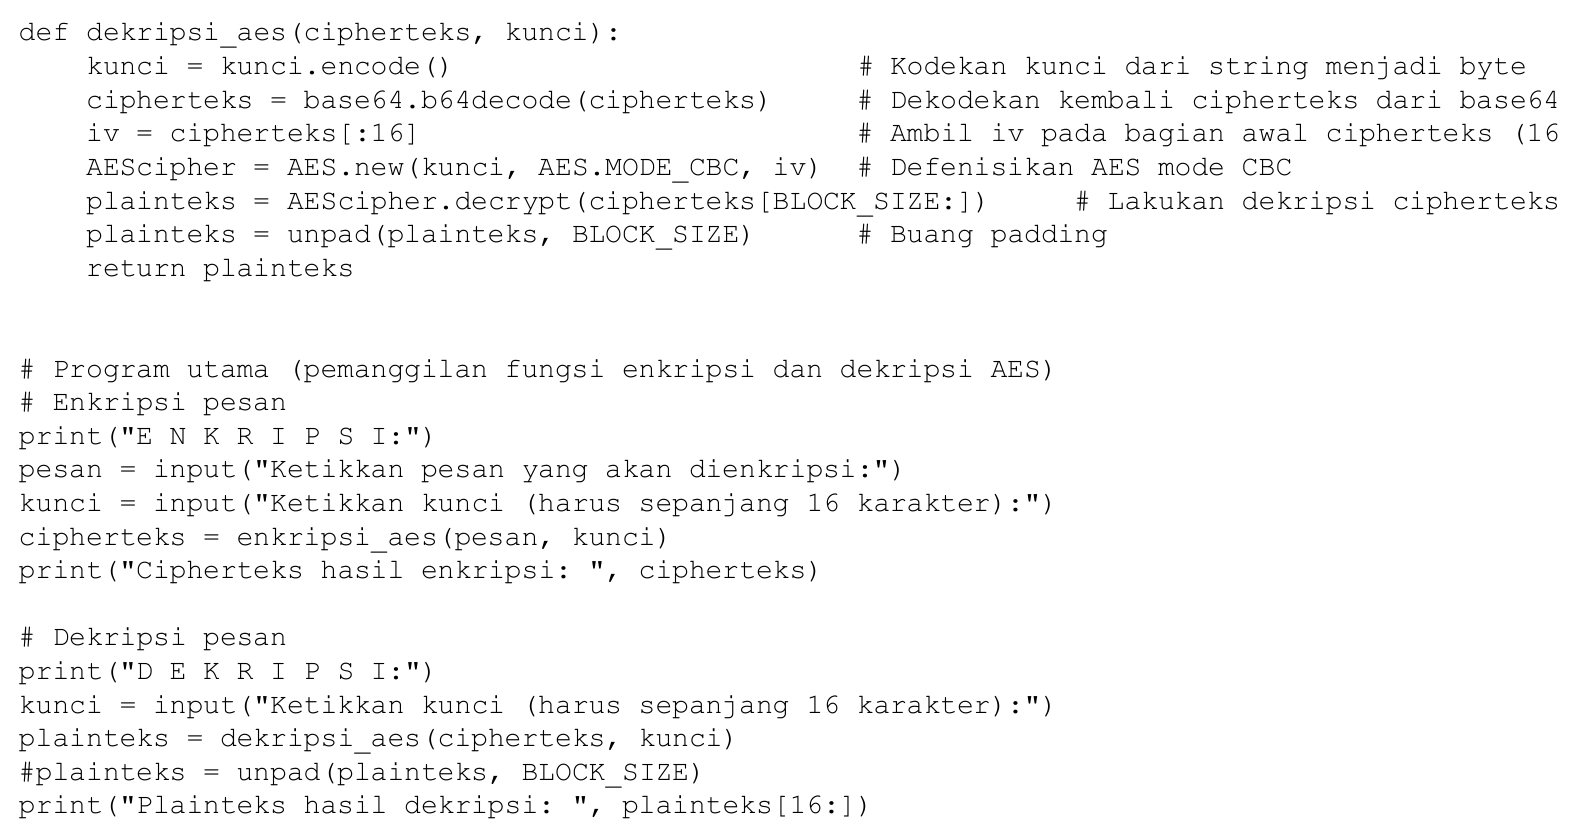
\includegraphics[width=172.20mm,height=228.69mm]{../../images/llm/page_047_img_01.png}%
\end{textblock*}

\end{document}
